\documentclass[a4paper,12pt]{article}
\usepackage[a4paper, total={180mm, 272mm}]{geometry}

\usepackage{fontspec}
\setmainfont[Path=fonts/, Extension=.ttf]{ipaexm}

\setlength\parindent{3.5em}
\setlength\parskip{0em}
\renewcommand{\baselinestretch}{1.247}

\usepackage{eepic}

\usepackage{tikz}

\begin{document}

\thispagestyle{empty}

\Large
\noindent \\
Level Auto Ino\medskip
\par
\normalsize
Spread the brightness range of the picture.\\
\par
It performs an automatic level correction, useful for increasing the image\par 
brightness and contrast.\\
\par
Based on the brightest and darkest values of the input image, the brightness\par 
range is expanded to the darkest (Out Min) and brightest (Out Max) values.\par
-{-}> See Figure 1: \textquotedbl Auto Levels - Calculation Diagram\textquotedbl\\
\par
Since it expands the range of each RGBA channel, it does not take into account\par
the RGBA\textquotesingle s balance. Therefore please note that it may change colors, in a colored\par
image.\\
\par
When checking the results, sub-camera must not be used.\par
Since the sub-camera input image range is different, its darkest and brightest\par 
values are different of those of the input image, and will give different results.\\
\\
-{-}- \ Inputs \ -{-}-\\
Source\par
Connect the image to be processed.\\
\\
-{-}- \ Settings \ -{-}-\\
In Min Shift\\
In Max Shift\par
The minimum and maximum values of the input image pixels are automatically\par calculated and adjusted by adding to their values.\par
For example, if there is only one bright pixel that needs to be ignored,\par
it is possible to spread the range by specifying a negative value for\par 
\textquotedbl In Max Shift\textquotedbl \ .\par
Pixel values (8 or 16 bits) are specified ranging from 0 to 1.\par
Minimum value is -1, maximum value is 1.\par
\noindent \hskip 7em Min \ \ \ \ \, 0\par
\noindent \hskip 7em Max \ \ \ \ -1\par
These values will make the screen become black.\par
\noindent \hskip 7em Min \ \ \ \ \, 1\par
\noindent \hskip 7em Max \ \ \ \ \ 0\par
These values will make the screen become white.\par
If both values are set to 0, there will be no adjustment by shift.\par
The default values for both are 0.\\

\newpage

\ \vspace{-0.2em}

\par
\noindent Out Min\par
\noindent Out Max\par
Determines the darkest (Out Min) and the brightest (Out Max) values of the output\par
image.\par
Minimum value is 0, maximum value is 1.\par
The defaults values are\par
\noindent \hskip 7em Out Min: 0\par
\noindent \hskip 7em Out Max: 1\\
\\
Gamma\par
Perform gamma correction between \textquotedbl Out Min\textquotedbl \ and \textquotedbl Out Max\textquotedbl .\par
A value between 0.1 and 1.0, will make the image become darker.\par
When the value is 1.0, no correction will be performed.\par
A value between 1.0 and 10.0, will make the image become brighter.\par
The default value is 1.\\
\\
Figure 1: Auto Levels - Calculation Diagram

\large
\noindent \begin{picture}(0,0)
\linethickness{0.01em}
\put(18.5,-94){\line(0,-1){81}}
\put(18.5,-94){\line(-2,-3){4}}
\put(18.5,-94){\line(2,-3){4}}
\put(18.5,-175){\line(-2,3){4}}
\put(18.5,-175){\line(2,3){4}}

\put(114,-22){\line(0,-1){199}}
\put(256,-22){\line(0,-1){199}}
\put(85,-51){\line(1,0){199}}
\put(85,-193){\line(1,0){199}}

\put(101,-7){\small{IN}}
\put(233,-7){\small{OUT}}
\put(290,-51){\small{1}}
\put(290,-193){\small{0}}
\put(72,-91){\small{max}}
\put(258,-69){\small{max}}
\put(116,-105){\small{max\_shift}}
\put(116,-176){\small{min\_shift}}
\put(72,-188){\small{min}}
\put(258,-188){\small{min}}
\end{picture}\\[3em]

\noindent \hskip 3.8em 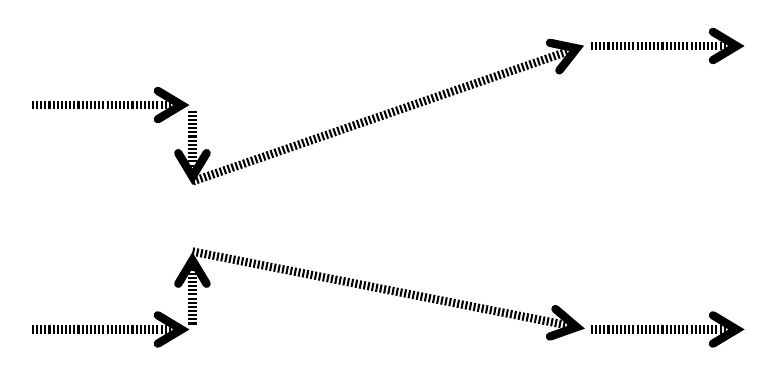
\begin{tikzpicture}[line width=3pt]
\draw[line cap=round] (1.6,-0.75) -- (1.9,-0.93) -- (1.6,-1.11);
\draw[dashed,dash pattern=on 0.75pt off 0.75pt] (0,-0.93) -- (1.9,-0.93);

\draw[line cap=round] (8.65,0) -- (8.95,-0.18) -- (8.65,-0.36);
\draw[dashed,dash pattern=on 0.75pt off 0.75pt] (7.1,-0.18) -- (8.95,-0.18);

\draw[line cap=round] (1.6,-3.6) -- (1.9,-3.78) -- (1.6,-3.96);
\draw[dashed,dash pattern=on 0.75pt off 0.75pt] (0,-3.78) -- (1.9,-3.78);

\draw[line cap=round] (8.65,-3.6) -- (8.95,-3.78) -- (8.65,-3.96);
\draw[dashed,dash pattern=on 0.75pt off 0.75pt] (7.1,-3.78) -- (8.85,-3.78);

\draw[line cap=round] (1.86,-1.54) -- (2.04,-1.84) -- (2.22,-1.54);
\draw[dashed,dash pattern=on 0.75pt off 0.75pt] (2.04,-1) -- (2.04,-1.84);

\draw[line cap=round] (1.86,-3.2) -- (2.04,-2.9) -- (2.22,-3.2);
\draw[dashed,dash pattern=on 0.75pt off 0.75pt] (2.04,-2.9) -- (2.04,-3.74);

\draw[line cap=round] (6.58,-0.14) -- (6.92,-0.21) -- (6.7,-0.49);
\draw[dashed,dash pattern=on 0.75pt off 0.75pt] (2.04,-1.9) -- (6.92,-0.21);

\draw[line cap=round] (6.65,-3.52) -- (6.92,-3.75) -- (6.58,-3.87);
\draw[dashed,dash pattern=on 0.75pt off 0.75pt] (2.04,-2.79) -- (6.92,-3.75);

\end{tikzpicture}

\end{document}